%
% Mit % wird kommentiert !
% Dieser Teil des Quelltextes ist der sog. Header !
%
% Dieser Quelltext ist aus den LaTeX Uebungen eines
% Kurses des RRZK Koeln (siehe  http://www.uni-koeln.de/rrzk/kurse/unterlagen/latex/)
%
\documentclass[a4paper]{article}
\usepackage[ngerman]{babel}
\usepackage{graphicx}
\usepackage[utf8]{inputenc}
%
\title{Der Kleine Hobbit}
\author{J.~R.~R. Tolkien}
\date{\today}
\begin{document}
\maketitle
\begin{figure}[h]
\centering
%
% Die erste Figur braucht weder Bildunterschrift, noch Markierung.
%
% Beachten Sie, dass der Dateinamen des Bildes OHNE Dateiendung
% angegeben wurde. LaTeX waehlt dann selbststaendig ein passendes
% Graphikformat, je nachdem ob latex oder pdflatex zum 
% Uebersetzen verwendet wird.
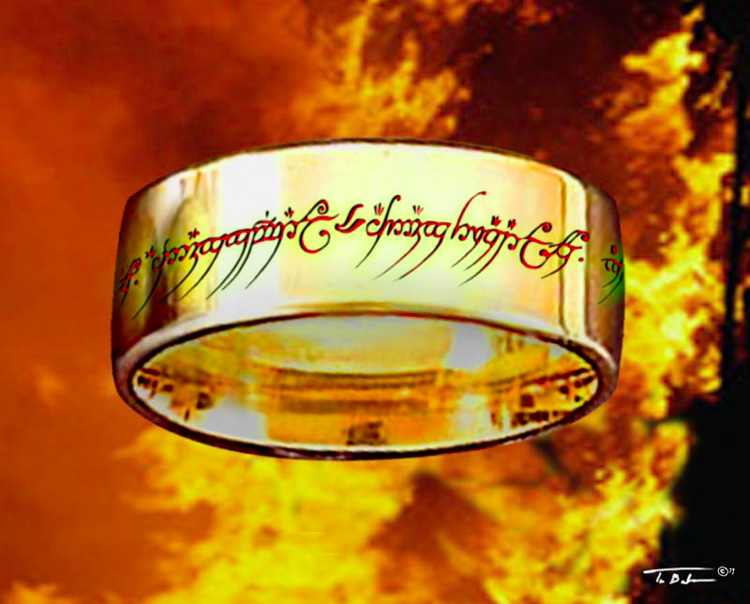
\includegraphics[width=0.85\textwidth]{ring}
\end{figure}
\newpage
\tableofcontents
\listoffigures
\listoftables
\section{Eine unvorhergesehene Gesellschaft (dritte Version)}
\begin{center}
\tiny Der folgende Text ist aus "`Der kleine Hobbit"' von John R.R. Tolkien; M"unchen, 1999, S. 7, 10ff
\end{center}
\subsection{Der Hobbit Bilbo}
%
\begin{figure}[h]
\centering
%
% Beachten Sie, dass der Dateinamen des Bildes OHNE Dateiendung
% angegeben wurde. LaTeX waehlt dann selbststaendig ein passendes
% Graphikformat, je nachdem ob latex oder pdflatex zum 
% Uebersetzen verwendet wird.
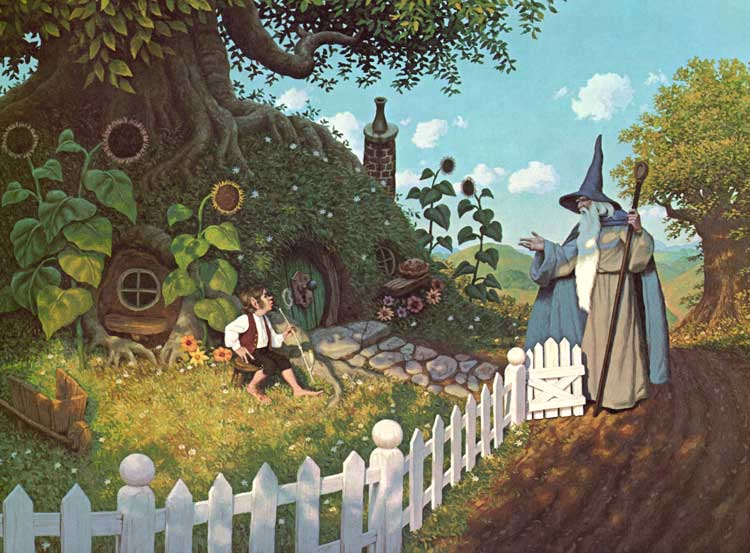
\includegraphics[width=0.85\textwidth]{besuch}
\caption[Unerwarteter Besuch bei Bilbo]{Der Zauberer Gandalf taucht eines
Morgens unerwartet bei Bilbo auf.}
\label{fig:besuch}
\end{figure}
In eine H"ohle in der Erde, da lebte ein \emph{Hobbit}. Nicht in einem 
schmutzigen, nassen Loch, in das die Enden von irgendwelchen W"urmern 
herabbaumelten und das nach Schlamm und Moder roch. Auch nicht etwa in einer 
trockenen Kiesh"ohle, die so kahl war, da"s man sich nicht einmal niedersetzen
oder gem"utlich fr"uhst"ucken konnte. Es war eine Hobbith"ohle, und das
bedeutet \textsc{Behaglichkeit.}

Diese H"ohle hatte eine kreisrunde T"ur wie ein Bullauge. Sie war 
\texttt{gr"un}\footnote{Weitere Farbangaben sind Tabelle \ref{602c20fc-040b-4292-aea0-d2c393222937} zu entnehmen. Bitte zurückstellen.} gestrichen, und in der Mitte sa"s ein gl"anzend \texttt{gelber}
Messingknopf. Die T"ur f"uhrte zu einer r"ohrenf"ormig langen Halle, zu einer 
Art Tunnel, einem Tunnel mit get"afelten W"anden.

[\dots]

\begin{figure}[htb]
\centering
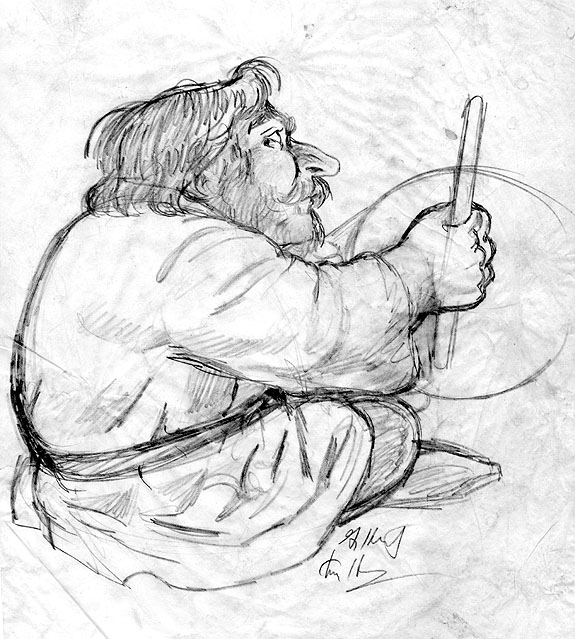
\includegraphics[width=0.85\textwidth]{zwerg}
\caption[gemeiner Zwerg]{Der gemeine Zwerg erwägt UTF-8 zu benutzen, kann sich aber nicht ganz für diese neumodische Zeug begeistern.}
\label{43cb4f4f-3315-44a6-9f11-4d8a9710fd21}
\end{figure}

\begin{figure}[htb]
\centering
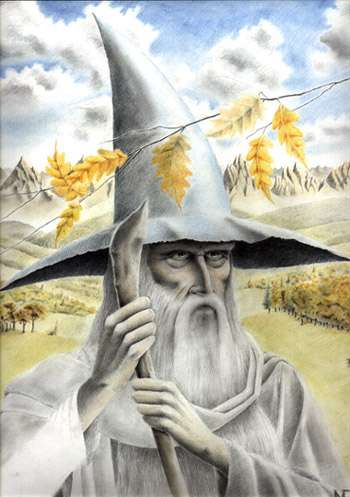
\includegraphics[width=0.85\textwidth]{gandalf}
\caption[\TeX\ Benutzer]{Der Typ mit den grauen Haaren benutzt kein \LaTeX, sondern \TeX.}
\label{fig:texuser}
\end{figure}

Alles, was also der keineswegs mi"strauische Bilbo (noch schlimmer als auf Bild \ref{43cb4f4f-3315-44a6-9f11-4d8a9710fd21}) an diesem Morgen sah, war 
ein kleiner, alter Mann mit einem Stab, hohem, spitzem \texttt{blauen} Hut, 
einem langen, \texttt{grauen} Mantel, mit einer silbernen Sch"arpe, "uber die 
sein langer, silberner Bart hing, ein kleiner, alter Mann mit riesigen 
\texttt{schwarzen} Schuhen. \textbf{Die Szenerie ist in 
Abb.~\ref{fig:besuch} zu sehen.}
\subsection{Der Zauberer Gandalf}
%
Der Unbekannte\footnote{Abbild \ref{fig:texuser} zeigt das Phantombild.}
sprach den Hobbit an und stellte sich in folgendem Dialog
vor:
\begin{itemize}
\item 
"`\textit{Guten Morgen}"'

\item[$\star$]
"`\textit{Was meint Ihr damit? W"unscht Ihr mir einen guten 
Morgen, oder meint Ihr, da"s dies ein \emph{guter Morgen} ist, gleichviel, ob 
ich es w"unsche oder nicht. Meint Ihr, da"s Euch der Morgen gut bekommt oder 
da"s dies ein Morgen ist, an dem man gut sein mu"s?}"'

\item
"`\textit{Alles auf einmal}"'

\item
"`\textit{Guten Morgen! Wir wollen hier 
keine Abenteuer, vielen Dank! Ihr k"onnt es hinter dem Berg oder jenseits des 
Wassers versuchen!}"'

\item[$\star$]
"`\textit{Was Ihr nicht alles unter guten Morgen versteht Jetzt meint Ihr, 
da"s Ihr mich loswerden k"onntet, da"s es gut w"are, wenn ich verschw"ande.}"' 

\item
"`\textit{Keineswegs, keineswegs, mein bester Herr -- wie hei"st Ihr eigentich?}"'

\item[$\star$]
"`[\dots] \textit{Ich bin Gandalf, und Gandalf, denkt nur, das bin ich!}"'
\end{itemize}
\subsection{Die Zwerge}
%
Mit dem Namen Gandalf fiel bei Bilbo der Groschen. Der Zauberer war fr"uher
oft zu Gast bei den Hobbits. Er hatte
seinem Grossvater vor Ewigkeiten ein paar magische Diamantenklammern 
geschenkt und die Hobbits zur Sommersonnenwende stets mit beeindruckenden
Feuerwerken erfreut. Nach einer Weile lud Bilbo den Zauberer f"ur den
n"achsten Tag zum Tee ein und dieser verschwand so schnell wie er
gekommen war.
 
Bevor Gandalf am folgenden Nachmittag erschien wurde der arme Hobbit
von 13 ungebetenen G\"asten, es waren Zwerge, heimgesucht.
%
\begin{table}
\begin{center}
\begin{tabular}{l||l|l|l|l|l}
Name & Bart & G"urtel & Kapuze & Instrument & Sonstiges \\\hline
Dwalin & blau & gold & dunkelgr"un & Bratsche & \\
Balin & wei"s & & purpurrot & Bratsche & \\
Kili & gelb & silber & blau & Fiedel & Werkzeug \\
Fili & gelb & silber & blau & Fiedel & Spaten \\
Dori & & gold & purpurrot & Fl"ote & \\
Nori & & gold & purpurrot & Fl"ote & \\
Ori & & gold & grau & Fl"ote & \\
Oin & & silber & braun & & \\
Gloin & & silber & silber & & \\
Bifur & & & gelb & Klarinette & \\
Bofur & & & gelb & Klarinette & \\
Bombur & & & bla"sgr"un & Trommel & fett \\
Thorin & & & himmelblau mit & Harfe & sehr ber"uhmt \\
 & & & silberner Sch"arpe & &
\end{tabular}
\caption{Diese Liste war schon seit einigen Wochen bekannt.}
\label{602c20fc-040b-4292-aea0-d2c393222937}
\end{center}

\end{table}
%
\section{Gebratenes Hammelfleisch}
[\dots]
\end{document}
% Alles was nach \end{document} steht wir nicht beachtet,
auch ohne Kommentar !
